\documentclass[a4paper, 11pt]{article}
\usepackage{geometry}
\usepackage{indentfirst}
\usepackage{setspace}
\usepackage{amsmath}
\usepackage{amssymb}
\usepackage{graphicx}
\usepackage{wrapfig}
\usepackage{caption}
\usepackage{indentfirst}
\setlength{\parindent}{20pt}
\usepackage{amssymb}
\usepackage{float}
\usepackage{subcaption}

\usepackage[backend=biber,style=ieee, sorting=none, sortlocale=en_US]{biblatex}
\bibliography{biblio.bib}

\graphicspath{ {./images/} }
\geometry{left=2.5cm, right=2.5cm, top=2.5cm, bottom=2.5cm}

\begin{document}	
	\title{Essay - Cognition and Computation }
	\author{{\small Alexandre da Rocha Rodrigues (2039952)}}
	\date{\today}
	\maketitle
	
	\section{Introduction}
	
		The EMNIST\cite{emnist} Balanced dataset is a more complete letter recognition dataset.
		The balanced slip has 47 classes - digits (0-9), uppercase letters (A-Z), some lowercase letters (a,b,d,e,f,g,h,n,q,r,t), a total of 131600 samples....
		
			
		a Deep Belief Network is a stack of Restricted Boltzmann Machines, another kind of energy-based model;
		they are unsupervised deep learning architectures that learn a probability distribution that could have generated the training data;
		this means they can be used to run both forwards and backwards passes through the architecture, to compute either hidden representations, or "prototypical" examples of a class based on the learned probability distributions;
		they are trained using an algorithm called contrastive divergence, whose goal is to reduce the difference between the learned probability distribution and the true one.
		
	
	\section{Hyper Parameters}
		After some testing, I used a DBN with 2 hidden layers of size 1000 and compared it with a similar FFNN.
		The best found parameters where: k = 1 (...), learning rate of 0.1 without decay (...), 
		Constant momentum of 0.9.
		Weights decay of 0.00001 
		.........
		
		These parameters were isolated and tested, i.e. starting from the 1st lab parameters, I changed only one of the parameters and found the best value, did this for all parameters and use the best of each in this final combination.
		This, obviously does not guarantee the best results, because the parameters can be the best when isolated but not the best combination of all of them.
		We can although consider these values as a good approximation to the best case.
		The objective was to reduce the average reconstruction error in the DBN training phase.
		
		
		
		
		
		
		
		
	\section{Results}	
			The DBN took 474 seconds to train (7 minutes and 53 seconds).
			The Perceptron was trained in 453 seconds (7 minutes and 33 seconds).
			The FFNN was trained in 60 epochs to achieve a training time close to the sum of the DBN and Perceptron training time, 932 seconds (15mins 32 secs).
			
			
	
	
		\subsection{Representations}
			
			\begin{figure}[H]
				\centering
				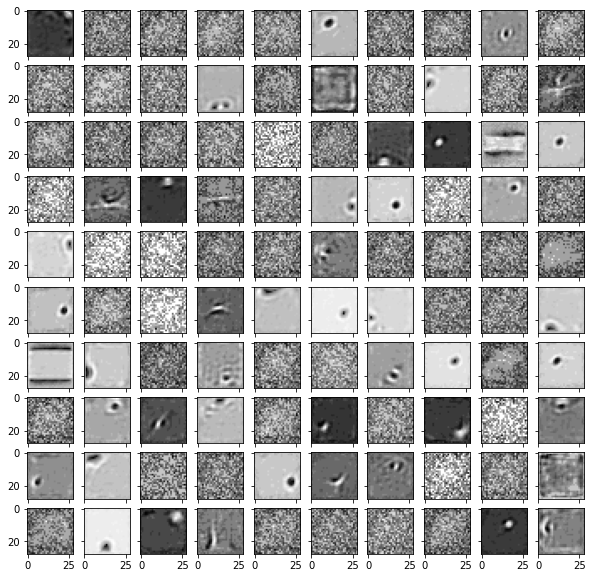
\includegraphics[width=.7\linewidth]{0.1_1.png}  
				\caption{Representation of the 1st hidden layer}
				\label{fig:rep1}
			\end{figure}
			
			\begin{figure}[H]
				\centering
				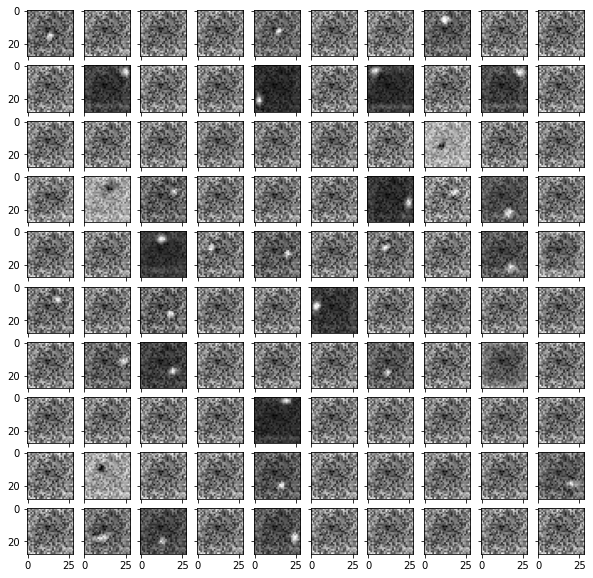
\includegraphics[width=.7\linewidth]{0.1_2.png}  
				\caption{Representation of the 2nd hidden layer}
				\label{fig:rep2}
			\end{figure}
			
			These results show ...
		
		\subsection{Dendrograms}
		
			\begin{figure}[H]
				\centering
				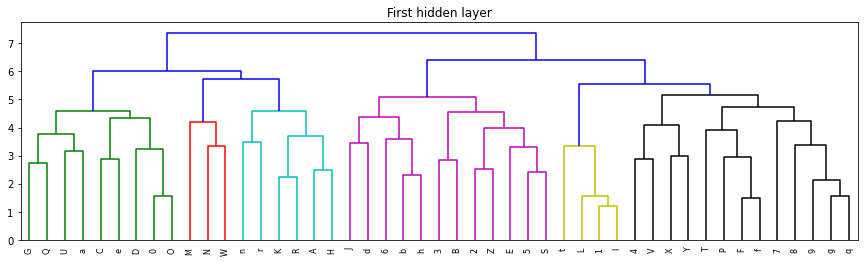
\includegraphics[width=.99\linewidth]{dend1.png}  
				\caption{Dendrogram for 1st hidden layer}
				\label{fig:dend1}
			\end{figure}
		
			\begin{figure}[H]
				\centering
				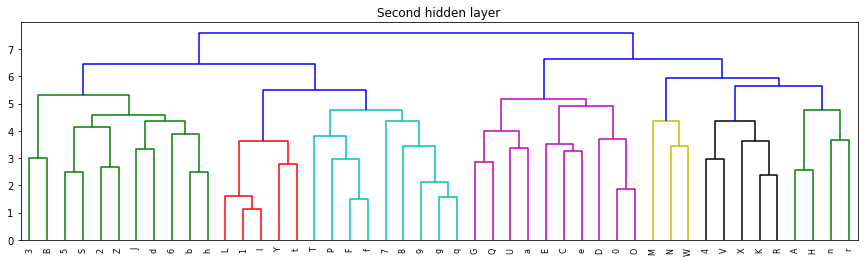
\includegraphics[width=.99\linewidth]{dend2.png}  
				\caption{Dendrogram for 2nd hidden layer}
				\label{fig:dend2}
			\end{figure}
		
			These results show ...
		
		
		
		
		
		\subsection{Confusion Matrix}	
			\begin{figure}[H]
				\centering
				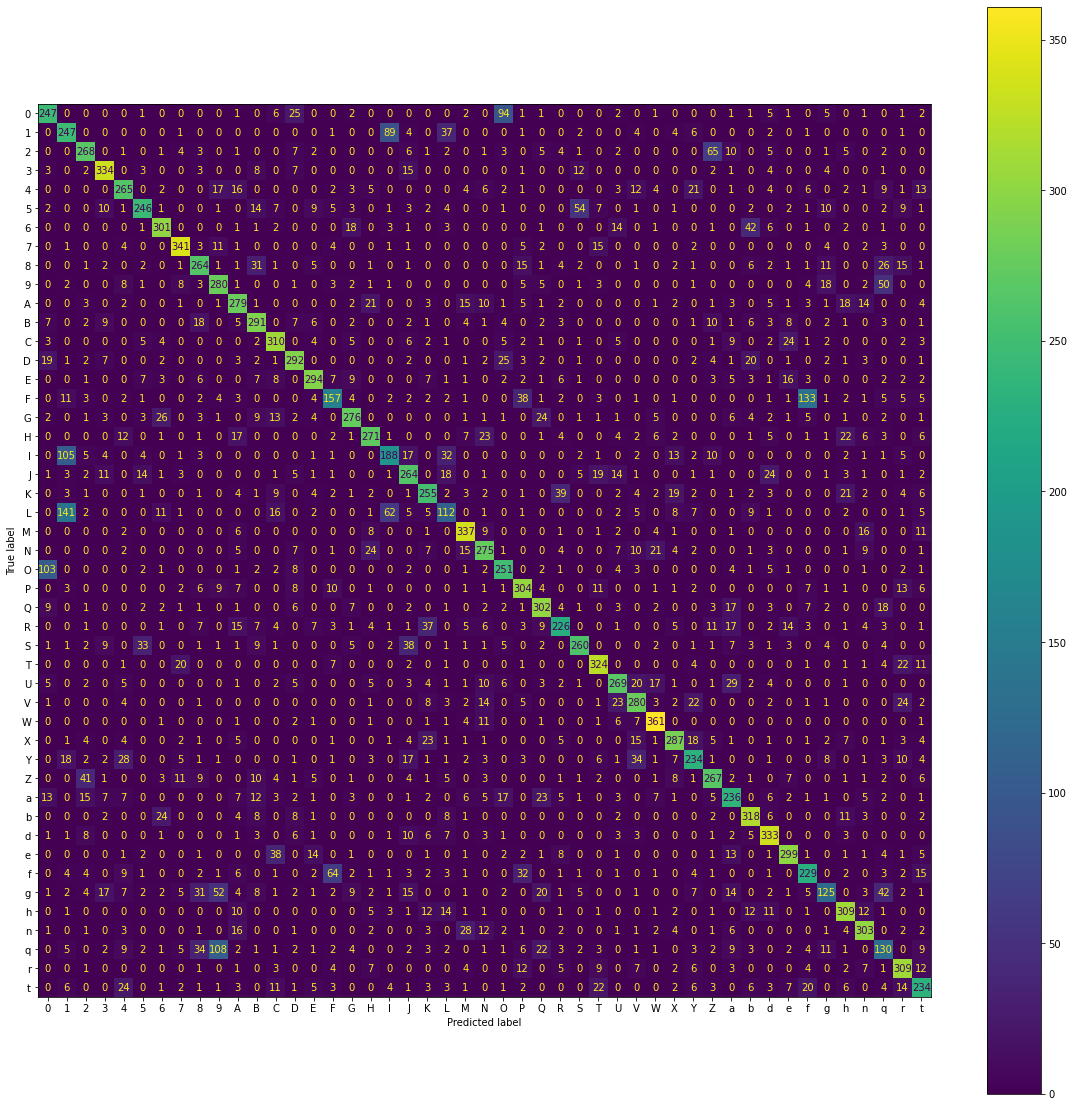
\includegraphics[width=.7\linewidth]{confmat.png}  
				\caption{Confusion Matrix}
				\label{fig:confmat}
			\end{figure}
			We can clearly see the similarities between letters as an human expects.
			"q" and "9", "L" and "1" .....
			
		
		
		
	\section{References}
		
		\printbibliography
		
		
	
	
	
	
	
	
			
\end{document}



